It will be shown later that the implementation of the spatial and temporal integration of the \emph{cable equation} that describes the time evolution of voltage in a cell accounts for over 99\% of all wall time. The discussion of \emph{the algorithm} here offers a basic mathematical description of the algorithm with many details that do not affect the implementation ommitted.

%%%%%%%%%%%%%%%%%%%%%%%%%%%%%%%%%%%%%%%%%%%%%%%%%%%%%%%%%%%%%%%%%%
\subsection{Discretization of The 1D Cable Equation}
%%%%%%%%%%%%%%%%%%%%%%%%%%%%%%%%%%%%%%%%%%%%%%%%%%%%%%%%%%%%%%%%%%
The partial differential equation (PDE) that describes the time evolution of the voltage at each node a discretized cell has the following general form:
\begin{equation}
     C\pder{V}{t} + I = f \pder{}{x} \left( g\pder{V}{x} \right)
\end{equation}
where $f$ and $g$ are functions of the spatial dimension $x$ (they are functions of \emph{cable radius} in this model). The value of current $I$ and capacitance $C$ are both dependent on the voltage $V$.

See \ap{appendix:discretization} for a detailed derivation of the spatial and temporal discretization. The discretization gives rise to a tridiagonal system of linear equations that is solved at every time step. The equation at each point has the following form,
\begin{equation}
    \at{a} \atplus{V}^{n+1} + \at{d} \at{V}^{n+1} + \at{b} \atminus{V}^{n+1} = \at{r}
\end{equation}
where the diagonals in the matrix are defined
\begin{align}
    \text{ upper diagonal : }  \at{a}  &=  -\frac{\at{f}\atplushalf{g}}{2\dx^2}, \nonumber \\
    \text{ lower diagonal : }  \at{b}  &=  -\frac{\at{f}\atminushalf{g}}{2\dx^2}, \nonumber \\
    \text{       diagonal : }  \at{d}  &=  \frac{\at{C}}{\dt} - ( \at{a} + \at{b} ), \nonumber \\
    \text{right hand side : }  \at{r}  &=  \frac{\at{C}}{\dt} \at{V}^n
                - \at{I}
                - \at{a} \left( \atminus{V}^{n} - \at{V}^{n} \right)
                - \at{b} \left( \atplus{V}^{n}  - \at{V}^{n} \right). \nonumber
\end{align}

The off-diagonal coefficients in the linear system, i.e. $\at{a}$ and $\at{b}$,  are constant in time because they depend only on the radius of the cable. In practice the off-diagonal entries in $\vv{a}$ and $\vv{b}$ are computed once at start up. The values on the diagonal and right hand side vector, i.e. those in $\vv{d}$ and $\vv{r}$ are updated at each time step, then modified when solving the linear system using Thomas' algorithm. The values on the diagonal and right hand side vector are calculated using the precomputed values for $\at{a}$ and $\at{b}$.
%%%%%%%%%%%%%%%%%%%%%%%%%%%%%%%%%%%%%%%%%%%%%%%%%%%%%%%%%%%%%%
\subsection{Trees and Branching}
%%%%%%%%%%%%%%%%%%%%%%%%%%%%%%%%%%%%%%%%%%%%%%%%%%%%%%%%%%%%%%
Here the one-dimensional discretization in the previous section will be extend to include branching, whereby the spatial domain is composed of a series of one-dimensional \emph{sections}, that are joined at branch points to form a tree.

A small tree structure that will be used throughout this section is illustrated in \fig{fig:tree}(a). It is important to note that the graph formed by the branching sections is a true tree, i.e. it has no circuits (once a section has branched, the branches can not ``rejoin'').

\begin{infobox}{Terms used describing discretization of trees}
\begin{itemize}[leftmargin=*]
    \item \textbf{section} a branch in the tree structure, which corresponds to the one-dimensional line segment between branch points. These are numbered $s*$ in \fig{fig:tree}(a).
    \item \textbf{branch} same definition as section.
    \item \textbf{node} a point in the spatial discretization. These are numbered in \fig{fig:tree}(b).
    \item \textbf{branch node} a node where two branches join. These are the blue points denoted $n*$ \fig{fig:tree}(a).
\end{itemize}
\end{infobox}

\begin{myfigure}{example of numbering of nodes and branches}{fig:tree}
\begin{center}
\includegraphics[width=0.6\textwidth]{./images/tree.pdf}
\\{\normalsize (a)}\\
\includegraphics[width=\textwidth]{./images/discrete_a.pdf}
\includegraphics[width=\textwidth]{./images/discrete_b.pdf}
\includegraphics[width=\textwidth]{./images/discrete_c.pdf}
\includegraphics[width=\textwidth]{./images/discrete_d.pdf}
\includegraphics[width=\textwidth]{./images/discrete.pdf}
\\{\normalsize (b)}
\end{center}
(a) The high level branch and connection numbering scheme, with the branch nodes and sections numbered; (b) the numbering of individual nodes in the fully discretized domain with 5 segments per section.
\end{myfigure}

The first step of the spatial discretization is to discretize each one-dimensional section. Then the nodes are numbered using a scheme that gives the matrix a sparsity structure that allows the linear system to be solved in linear time, equivalent to Thomas algorithm.

A numbering scheme for the nodes that facilitates efficient solution of the linear system is not unique. A general description of a valid numbering strategy is as follows:
\begin{enumerate}
    \item
        One node is chosen as the \emph{root node} of the tree, either a terminal node or a branch node, and assigned index 1.
    \item
        The tree is then traversed along each branch with the root node as the starting point. The nodes are numbered sequentially in ascending order.
    \item
        Every node (except the root node) has one-and-only-one \emph{parent node}, which is its neighbour that is closer to the root node (and thus has a lower index).
\end{enumerate}
The key property that is maintained by the numbering scheme is that the index of a node's parent node is lower than the node's index (equivalent to \emph{minimum degree ordering}). An example of a numbering strategy being recursively applied to our example tree is shown in \fig{fig:tree}(b).

\begin{myfigure}{matrix sparsity pattern}{fig:sparsity}
\begin{center}
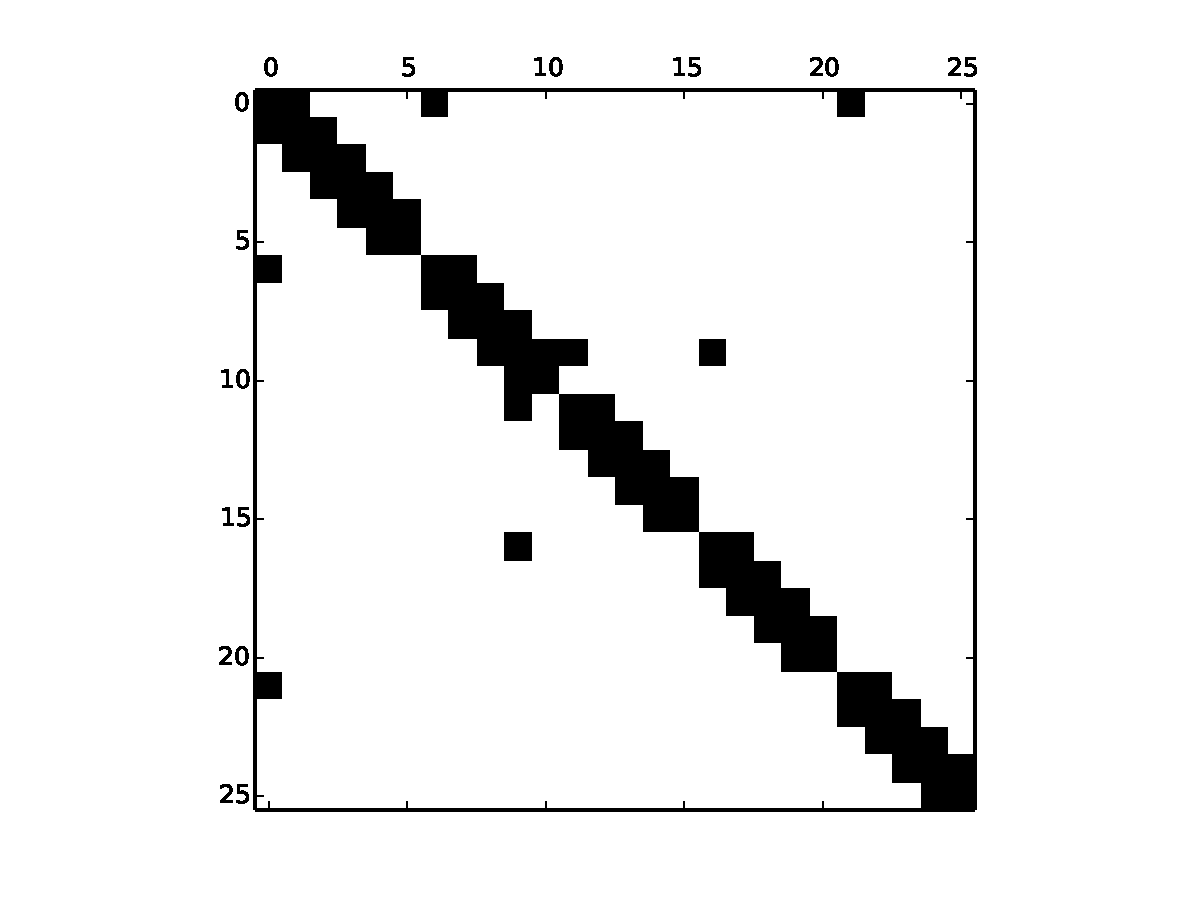
\includegraphics[width=0.5\textwidth]{./images/sparsity.pdf}
\end{center}
Sparsity pattern of the matrix corresponding to the tree numbering in \fig{fig:tree}.
\end{myfigure}

To describe the sparsity pattern of the matrix from this numbering only the parent indexes, $p_i\quad i\in[2:n]$, for each node need to be stored. The matrix sparsity pattern, which is illustrated for our example tree numbering in \fig{fig:sparsity}, has the following properties:
\begin{infobox}{Properties of the linear system}
\begin{itemize}[leftmargin=*]
    \item
        The sparsity pattern is symmetric.
    \item
        The diagonal values are all nonzero.
    \item
        There is exactly one off diagonal value in each row of the lower triangle at $a_{ik}$ and exactly one off diagonal value in each column of the upper triangle at $a_{ki}$, where $k=p_i$.
    \item
        The matrix can be stored with three vectors, $\vv{a}$, $\vv{b}$ and $\vv{c}$:
        \begin{align}
            a_i &= A_{ki} \\
            b_i &= A_{ik} \\
            d_i &= A_{ii}
        \end{align}
        where $k=p_i$.
\end{itemize}
\end{infobox}

\begin{note}
The choice of the root node and the traversal order when generating the numbering is important if trying to solve the linear system in parallel. It is possible to solve sub-trees that branch from a branch node independently, before combining the results to solve the value at the branch node. For sequential solution on the CPU this isn't important, however a GPU implementation might try to take advantage of this.
\end{note}
%%%%%%%%%%%%%%%%%%%%%%%%%%%%%%%%%%%%%%%%%%%%%%%%%%%%%%%%
\subsection{Hines Algorithm}
\label{sec:hines}
%%%%%%%%%%%%%%%%%%%%%%%%%%%%%%%%%%%%%%%%%%%%%%%%%%%%%%%%
These linear systems can be solved very efficiently, in linear $O(N)$ time, using an algorithm that is equivalent to the Thomas algorithm for solving tri-diagonal systems. This algorithm, called Hines algorithm, proceeds by eliminating the nonzero entries in the upper triangle of $A$. Recall the matrix property that there is only one non-zero value in each column of the upper triangle at $A_{ki}$, which is stored in $a_i$.
\begin{equation*}
\left(
        \begin{array}{ccc}
            A_{kk} & \dots      & A_{ki} \\
        \vdots     & \ddots     & \mathbf{0} \\
            A_{ik} & \mathbf{0} & A_{ii}
        \end{array}
\right)
\text{which is stored as:}
\left(
        \begin{array}{ccc}
            d_k & \dots      & a_i \\
        \vdots  & \ddots     & \mathbf{0} \\
            b_i & \mathbf{0} & d_i
        \end{array}
\right)
\end{equation*}
The nonzero value in column $i$, i.e. $a_i$, can be zeroed out with a row operation
\begin{equation*}
    \text{row}_k \leftarrow \text{row}_k - a_i/d_i\cdot\text{row}_i.
\end{equation*}
In practice the value of $a_i$ is not changed, and only the values in on the diagonal and in the RHS vector have to be modified
\begin{align}
d_k \leftarrow d_k - a_i/d_i\cdot b_i, \nonumber \\
r_k \leftarrow r_k - a_i/d_i\cdot r_i, \nonumber
\end{align}
So that our submatrix now looks like
\begin{equation*}
\left(
        \begin{array}{ccc}
            d_k - a_i/d_i\cdot b_i  & \dots      & \mathbf{0} \\
        \vdots                      & \ddots     & \mathbf{0} \\
            b_i                     & \mathbf{0} & d_i
        \end{array}
\right)
\left(
        \begin{array}{c}
            r_k - a_i/d_i\cdot r_i \\
        \vdots                     \\
            r_i
        \end{array}
\right)
\end{equation*}


The algorithm proceeds by eliminating the values in the upper triangle with a backward sweep over columns $n:-1:2$.
A forward sweep is then used to eliminate the nonzeros in the lower triangle, determine the solution.

\begin{note}
In practice, this algorithm is very efficient, contributing less than 1\% to the time to solution in the benchmarks released with the PCP. 
\end{note}


